% https://uwaterloo.ca/writing-and-communication-centre/cars-model-create-research-space (CaRS)
\section{Introduction}
% Move 1: Establish a Research Territory
%%%%%%%%%%%%%%%%%%%%%%%%%%%%%%%%%%%%%%%%%
The world around us is three-dimensional, but still the most common way to visualise data captured from this three-dimensional world is on a two-dimensional screen. Recent technological advancements within the area of head-mounted displays (HMD) have enabled many new applications across various domains to visualise and interact with 3D data. Applications can be found in areas such as healthcare~\cite{Buettner20}, environmental sciences~\cite{Rambach21}, education~\cite{FreinaOtt}, and construction~\cite{WangP18}.

These areas all benefit from the fact that immersive technologies, such as HMD technology, provide a unique \emph{medium} with great expressive, interactive and representative power~\cite{Rubio17}. With the aid of immersive visualisation, the user can be fully immersed within the 3D data providing an intuitive experience. Within the immersive visualisation, the user can manipulate the 3D scene easily by scaling, rotating and translating to get the best vantage point. The user experience can be further enhanced by incorporating analytical reasoning and decision making elements within the virtual environment; this paves the way towards immersive analytics~\cite{Chandler15}.
%Two mainstream technologies which enable immersive visualisation are a cave automatic virtual environment (CAVE) and a head-mounted display (HMD)~\cite{Cordeil17}.

Before immersive analytics can even be contemplated, the geometry of the physical world around needs to be captured first. A common data modality to accurately capture this, is point cloud data~\cite{Barber08}. Applications based on point cloud data have been on the rise in recent years~\cite{WangYanyun19, wang2019Applications}. This trend can be explained by the fact that the costs of sensor technology, storage and computing have been decreasing over recent years. Furthermore, the advent of autonomous vehicles have also provided a boost towards utilising this data modality. Autonomous vehicles use point cloud data to avoid collisions with other road users such as pedestrians, cyclists and other vehicles~\cite{LiIbanez20}.

Point clouds are usually captured by a laser scanning process, but other methods such as photogrammetry are also possible~\cite{Westoby12}. Laser scanning works by emitting a pulse of (usually) non-visible laser light and measuring the time-of-flight, this technique is called LiDAR. The time-of-flight is proportionally related to the distance to the object. Each captured reflection of a pulse will correspond to a point in 3D space; a collection of such points is called a point cloud. Generally speaking, laser scanning will achieve a higher accuracy compared to photogrammetry~\cite{Kalvoda20}. Though, this comes at the cost of more expensive hardware for laser scanning. The advantage of laser scanning is that it provides an immediate accurate 3D representation of the environment under varying illumination conditions. If the sensor platform carrying the laser scanning equipment is augmented with image sensors, it is also possible to add colour information to each captured point.

% Move 2: Establish a Niche - Brugje naar railway maken
%%%%%%%%%%%%%%%%%%%%%%%%%%%%%%%%%%%%%%%%%%%%%%%%%%%%%%%%%%%%%%
Within the rail domain, there has been an increasing interest in using point cloud data for various tasks. A few examples of these tasks include: automatic clearance inspection~\cite{ZhongDan20}, rail deformation monitoring~\cite{Karunathilake20}, identifying risk posing vegetation~\cite{Hoerbinger20}, foreign object detection~\cite{QuJinyan23}, and automatic rail infrastructure recognition~\cite{arastounia2015automated}. Despite these technological advancements, immersive visualisation of point cloud data and the derived information has not been explored for this domain.

% Move 3: Occupy the Niche
%%%%%%%%%%%%%%%%%%%%%%%%%%%%%%%%%%%%%%%%%%%%%%%%%%%%%%
Therefore the goal of this research is to explore the possibilities and challenges of immersive visualisation of point cloud data for the rail infrastructure domain. By reaping the benefits of immersive visualisations it is expected that the time to insight can be decreased and the user interaction experience can be improved. The work presented here is meant as a technological demonstrator to show the potential and to identify the open challenges of immersive visualisations using HMD technology. 

The work outlined here will follow the design science research methodology~\cite{peffers.07}. Design science focuses on creating and evaluating information technology artefacts~\cite{hevner.04}. The immersive visualisation application presented here is a perfect example of such an artefact. The key elements of this methodology are problem identification and motivation, objective definition, design and development, demonstration, evaluation, and communication. Problem identification and motivation are covered by the introduction and the related work section. The sections thereafter have a one-to-one correspondence to the remaining elements of the design science research methodology. Finally, it is worth noting that the manuscript in front of you covers the communication element.

\section{Related work}
Several diverse applications of immersive visualisation are highlighted in this section. The application areas cover archaeology and construction, smart cities, and point cloud annotation.

Within the area of archaeology, there is an increased interest in using immersive visualisations as well, and several use-cases have been presented. The geometry of the scene can be captured with point cloud data, whereas the visual appearance of the scene can be captured with high-resolution photos. For instance, the Istanbul \c{C}atalca \.{I}nce\u{g}iz Caves, Turkey have been digitally preserved this way and can now be explored within an immersive virtual visualisation~\cite{Buyuksalih20}.

Immersive visualisation can also provide the possibility to explore city centres from a different era. The work of \citeauthor{Tschirschwitz19} present a use-case were it is possible to explore the city of Duisburg, Germany from a 1566 perspective~\cite{Tschirschwitz19}. Also modern cities can benefit from the advancements within the area of point clouds and immersive visualisation. For instance \citeauthor{davis21} explore how accurate urban-scale 3D city models can be generated from point cloud data~\cite{davis21}. These city models can then be used for a large range of immersive applications, such as planning, design, training, and operations.

Another use-case of immersive point cloud visualisation is robotic telepresence. For instance, \citeauthor{Bruder14} use an unmanned robotic vehicle equipped with a laser scanner to scan and stream the captured environment in real-time to a remote location. At the remote location the user can explore the scene within an immersive visualisation~\cite{Bruder14}. This enables inspections or viewings at remote or dangerous locations.

Analysing data from autonomous driving experiments can be a daunting task. An autonomous vehicle will record an enormous amount of sensor data from a plethora of sensor devices such as camera, LiDAR, accelerometer, GPS, etc. In order to visualise these data, \citeauthor{Oliveira21} introduce a virtual reality based tool which is able to aggregate different data sources into a unified visualisation~\cite{Oliveira21}. This tool is able to visualise point clouds, bounding boxes of detected objects, images from the camera feed, and plots from diverse sensors.  

Within the architecture, engineering and construction (AEC) industry keeping track of construction progress and to monitor if what is built matches the original design is a cumbersome task. Therefore, \citeauthor{Vincke19} propose an immersive visualisation solution combining data from 3D models with point cloud data captured at the construction site~\cite{Vincke19}. Deviations between `as-build' and `as-designed' are visualised by colour-coding the captured point cloud based on the deviation. Challenges of this project were combining data from multiple sources and rendering large point clouds.

Virtual reality applications designed to annotate point cloud data are an active research topic requiring visualisation of and interaction with point cloud data. An important element of these applications is an expressive visualisation of the data and an intuitive user interaction for annotation. The work of \citeauthor{garrido2021point} makes use of a virtual environment in combination with a hand-held controller to make annotations. Within the virtual environment a size-adjustable sphere is used as a brush to add or delete points to the current selection~\cite{garrido2021point}. A similar approach was used by \citeauthor{Franzluebbers22} for the task of annotating cotton balls within high-resolution cotton plant scans~\cite{Franzluebbers22}. The work of \citeauthor{Doula22} focuses on placing bounding boxes around objects within a virtual environment. To do so, first the four corners of the base of the bounding box are placed using controllers, after which the box can be scaled and rotated to fit the object of interest~\cite{Doula22}. Note that all the before-mentioned examples make use of controllers. A common finding of these examples is that users found the immersive solution much easier to work with and faster compared to making annotations on a screen.

For a broader perspective of using virtual reality for visualisation the reader is directed to the extensive literature review of Korkut and Surer~\cite{Korkut23}.

Immersive visualisation of point cloud data has been explored for other domains, but not yet for the rail domain. The explorative study presented here is a first initial step towards immersive visualisations of point cloud data from the rail domain.

% DSRM: Define objectives of a solution
\section{Objectives}
There are two main objectives of this project. First objective was to create a demonstrator to showcase the possibilities of immersive visualisation and interactions of point cloud data. Second objective is to identify challenges and knowledge gaps during the creation process of this immersive visualisation application. These two objectives align well with a research- through-design methodology. This methodology states that with the creation of a research artefact, in this case an immersive visualisation application, also an appropriate conduit is established to elucidate the research findings~\cite{Zimmerman07}.

The use case presented here is related to the rail infrastructure domain. A train-mounted laser scanner is used to capture the environment as a point cloud. Part of this data are labelled~\cite{ton2024dataset} in order to train a machine-learning model to detect certain objects present in the railway environment. The following objects were annotated: street lights, signs, catenary arch masts, signals, tension rods and relay cabinets. Samples from this dataset have been used as use-case for the immersive visualisation application. Samples are stored in the open LASer (LAS) format~\cite{LASspec}.

A definitive set of objectives was drafted for the current prototype, based on expert interviews with two engineers from Strukton Rail, input from the principle investigator, and the associate lector of the Augmented Interaction research line. Based on the expert interviews, augmented reality was chosen because users would still be partially aware of their surroundings. Partial awareness is important when working in a collaborative office environment. The final set of objectives, based on the input from diverse experts, is listed below. Italicised objectives were not implemented due to time constraints and/or technical challenges.

\begin{itemize}
    \item Load point cloud data from LAS files.
    \item Use intuitive hand gestures to scale, rotate and move the scene.
    \item Meet the required 60 frames per second (FPS) for smooth viewing.
    \item Use a different colour for each of the object classes.
    \item Toggle visibility of certain object classes using voice commands.
    \item \textit{Display meta-data of an object when selected.}
    \item \textit{Automatic level of detail.}
    \item \textit{Use a `swiping' hand gesture to traverse through the point cloud scene from a train operator viewpoint.}
\end{itemize}

% DSRM: Design and development
\section{Design and development}
A suitable immersive visualisation technology must be selected. There are two mainstream technologies towards immersive visualisation: cave automatic virtual environment (CAVE) and a head-mounted display (HMD). The additional costs associated with the CAVE technology, do not outweigh the benefits when compared to HMD technology~\cite{Combe23, Cordeil17}. Based on this fact and the client's preference, the immersive visualisation technology chosen for this application was HMD. To be specific, the Microsoft HoloLens~2 was used as the target device as it was readily available at client's company and has a long standing track record within academia~\cite{Park21}.

To make use of this target device, a piece of middleware is required which renders point cloud data and enables interactions with the scene. For this purpose, the Unity platform was used to develop the immersive visualisation application as it is the most common platform for this task~\cite{Korkut23}. Additional factors to support his decision, were the presence of prior knowledge, the fact that the platform is freely available for students, and good support for a large range of extended reality hardware types. The Unity version used for development of the prototype was 2021.3.15f1.

To speed up the development of the application in Unity, an existing commercial Unity asset has been used to read the point cloud files. This asset, the \textit{Point Cloud Viewer and Tools v2.70}\footnote{\url{https://assetstore.unity.com/packages/tools/utilities/point-cloud-viewer-and-tools-16019}} is capable of reading different formats of point cloud data and supports a large number of points. Unfortunately, this library was not capable of reading the custom fields which had been added to the LAS files. These custom fields where used to encode the object class of a point. The existing code has been modified to support reading this custom data. Furthermore, threading has been implemented to speed up the loading of a point cloud file, with the `Unity Jobs System' package. Using threading the data loading throughput increased from 74~k points per second to 372~k points per second.

Due to memory limitations of the headset it was not possible to load large point clouds directly on the device. Instead holographic remoting was used. In this case, the application runs on an external host which also takes care of the rendering. The rendered images are then streamed to the HMD.

\subsection{Interaction}
Intuitive interaction plays an important role within immersive visualisation applications. Therefore the application supports multi-modal interactions using natural hand gestures and voice commands. Thus avoiding the need for controllers. The following hand gestures are supported:
\begin{itemize}
    \item Single hand for pinching and rotating the point cloud
    \item Two hands for scaling and moving the point cloud
\end{itemize}

The Unity engine uses box colliders to detect interactions with objects. These box colliders are invisible virtual objects within the scene and are used for triggering events. Each individual object of interest within the point cloud scene has its own box collider. To enable interactions with the entire scene, such as rotating and scaling, a box collider was present around the entire scene. 

The main menu and label menu can be activated by finger presses in augmented reality. The colour palette used for the menus was derived from the colours present in the Strukton logo.

Besides hand gestures, another option to toggle certain menus or object visibility within the scene is by voice commands. The following voice commands are currently supported:
\begin{itemize}
    \item ``Toggle main menu''
    \item ``Toggle label menu''
    \item ``Toggle \textless{}\textit{object}\textgreater'', where \textless{}\textit{object}\textgreater{} \(\in\) \{background, poles, relay cabinet, rod and foundation, signs, streetlights, signals\}
\end{itemize}
The ``Toggle \textless{}\textit{object}\textgreater'' voice commands enable or disable the visibility of the object in question.

% DSRM: Demonstration
\section{Demonstration}
This section demonstrates several aspects of the devised application. Fig.~\ref{fig:immvis:scale} shows a user performing the scaling task with both hands. The figure depicts a railway scene, the objects in green are catenary masts together with the tension rods.

\begin{figure}[htbp]
    \centering
    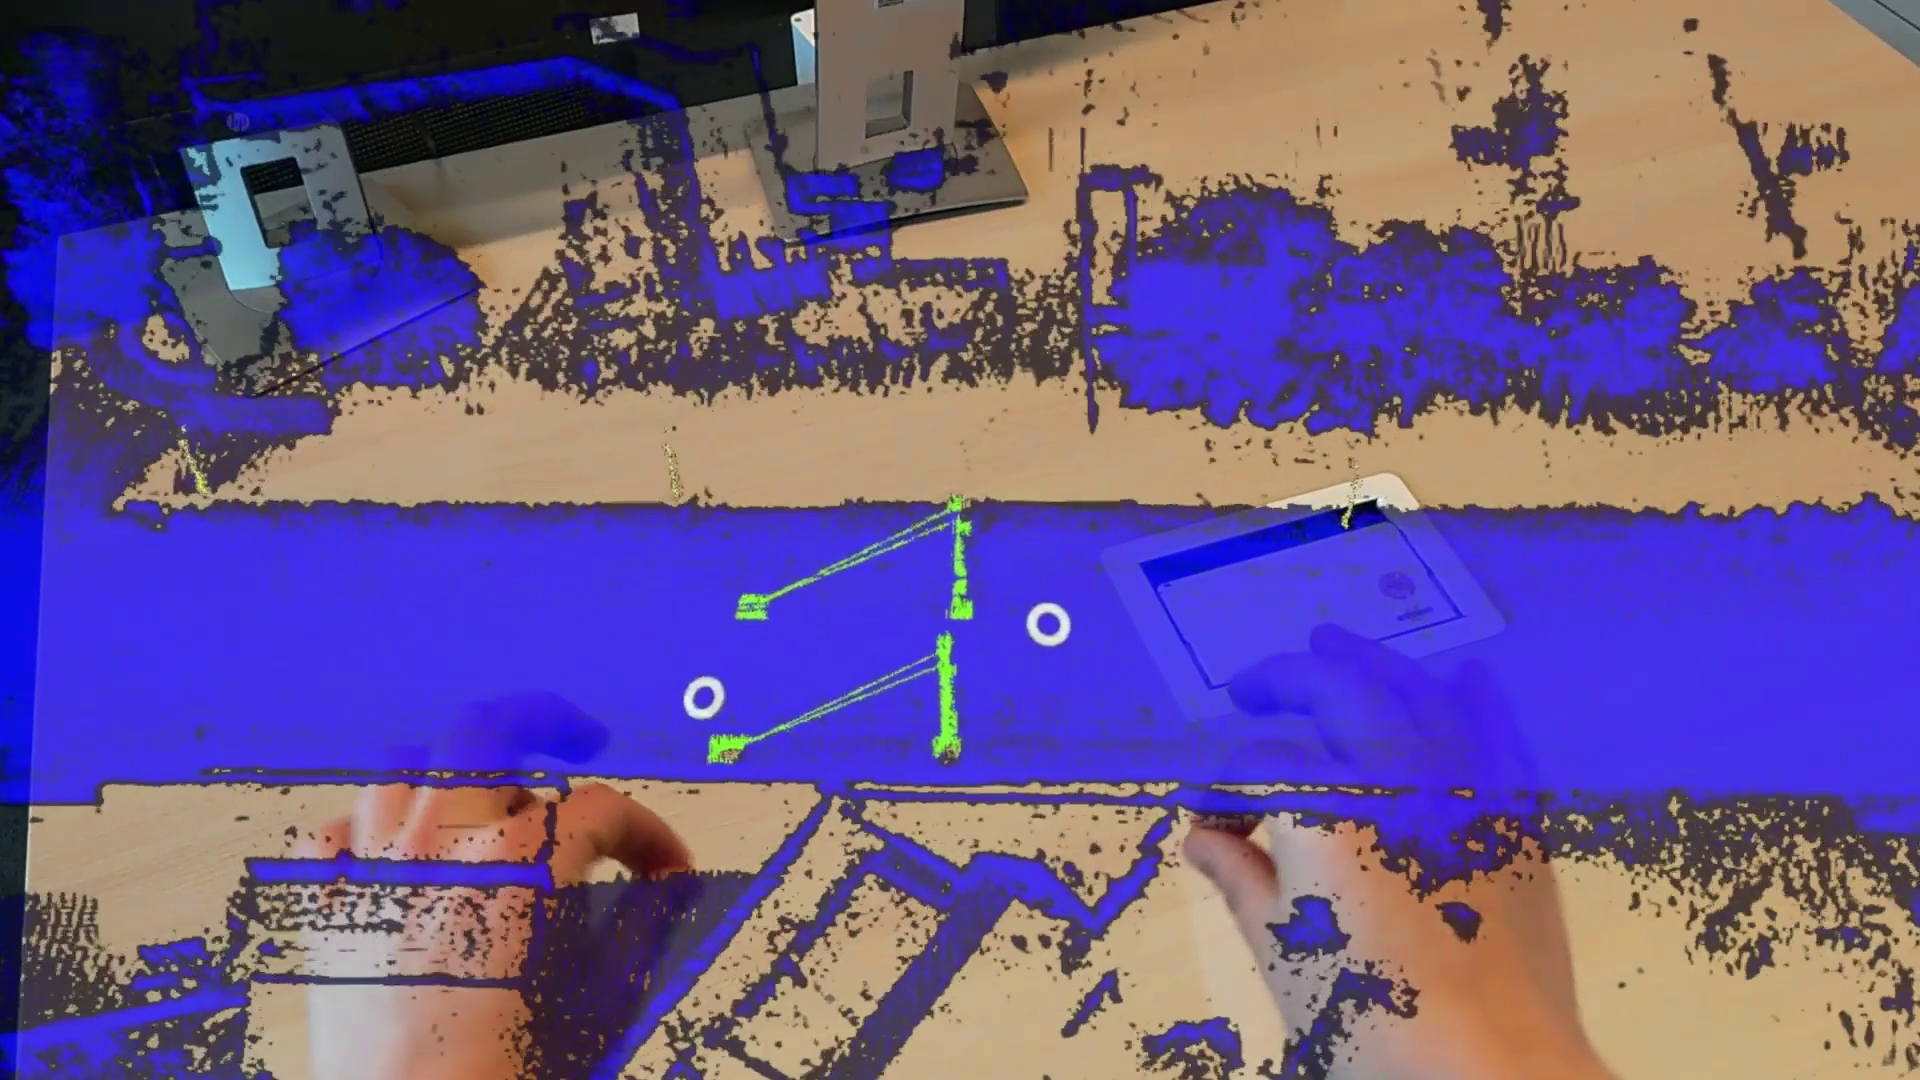
\includegraphics[width=0.7\linewidth]{./Chapters/immvis/figs/zoom_interaction.png}
    \caption{User performing the scaling task with both hands.} 
    \label{fig:immvis:scale}
\end{figure}

Several examples of the user interface are provided in Fig.~\ref{fig:immvis:ui}. The user interface on the left depicts the loading screen. During loading of the point cloud it shows a progress bar. The middle user interface shows the menu for toggling the visibility of certain objects within the scene. Due to time constraints all symbols are the same, but for a next iteration symbols should be designed to match the object categories. The user interface on the right shows the meta-data information about an object. Currently it shows mock data, but for a real application any information from an external data source can be shown here.

\begin{figure*}[!ht]
    \centering
    \begin{subfigure}{0.3\textwidth}
        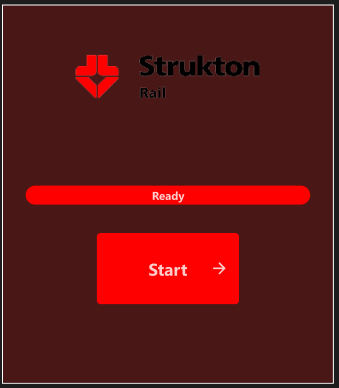
\includegraphics[width=\textwidth]{./Chapters/immvis/figs/Strukton_load.png}
        \caption{Loading screen}
    \end{subfigure}%
    \hfill
    \begin{subfigure}{0.3\textwidth}
        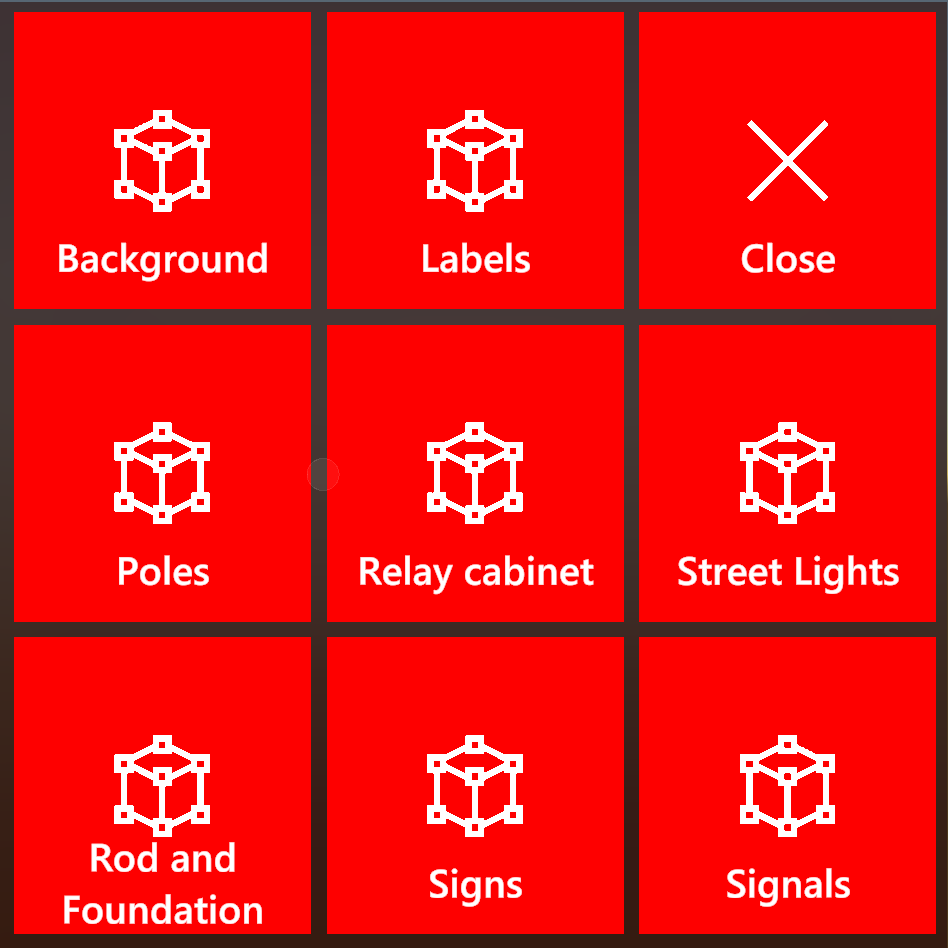
\includegraphics[width=\textwidth]{./Chapters/immvis/figs/Strukton_label-menu.png}
        \caption{Label menu}
    \end{subfigure}%
    \hfill
    \begin{subfigure}{0.3\textwidth}
        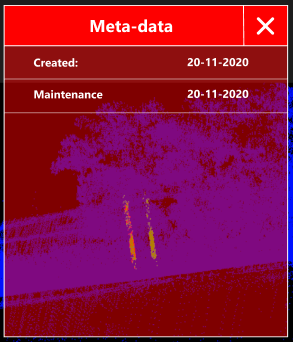
\includegraphics[width=\textwidth]{./Chapters/immvis/figs/Strukton_meta-data.png}
        \caption{Meta-data menu}
    \end{subfigure}%
    \caption{User interface examples.} 
    \label{fig:immvis:ui}
\end{figure*}

The current application has been tested on samples which span 75~m of railway track. Loading a single sample takes several seconds. Hence, the scalability and performance should be further improved. More detailed thoughts on this topic are provided in the \emph{Future work} section (see Section~\ref{sec:immvis:render}).

% DSRM: Evaluation
\section{Evaluation}
A small (\(n=6\)) user evaluation was done to evaluate the usability and user experience of the designed application. At first sight one would think that such a small number lacks sufficient convincing power. But, the model suggested by Nielsen and Landauer for estimating usability problems~\cite{Nielsen1993}, indicates that $\approx$~89\% of usability problems should be found. The user evaluation was conducted in a large, well lit office space. Participants were asked to perform certain task such as opening the main menu, toggling certain labels both manually and by voice control, and interacting with the point cloud. No prior information about the operation of the application was given to the participants, but if participants got stuck, they were helped out. During the evaluation participants were asked to think aloud. After the evaluation session, participants were asked to fill-out a small post-hoc questionnaire. Results from this post-hoc questionnaire, in combination with the observations and notes are categorised and summarised below.

\subsection{Point cloud interaction}
Rotation of the scene required participants to single-handedly pinch the scene and make a twisting motion with their hand. This method of rotating the scene was not intuitive for most participants, participants had the tendency to pinch the point cloud with both hands and make a rotating movement with both hands around a virtual origin of rotation. The single handed operation was also very sensitive, giving the participants the impression that the point cloud `stuck' to their hand. Making it prone to accidental movements and rotations.

Besides rotating the scene, participant were also asked to zoom in. When asked to zoom in, some participants had the tendency to use the same had gesture which commonly are used on smartphones. This gesture starts with the thumb and index finger pinched and in fluent motion the distance between index finger and thumb is expanded. This gesture is reversed when the goal is to zoom out. These gestures were not supported by the current application.

\subsection{Menu interaction}
The evaluation covered both the manual and voice based interactions with the menu. An intuitive location of the menu in virtual reality was challenging to determine. The participants remarked that the menu was too far away. Also the menu was placed at the edge of the field of view which was not ideal. Furthermore, the buttons were also placed too close together, making it prone to accidental presses. Some participants remarked that having some form of feedback when pressing a button would be nice. For instance an audible click or the highlighting of the button.

Another option to interact with the menu was by using voice commands. During evaluation it was discovered that the microphone used by the application was from the laptop and not the headset. By moving the laptop closer to the participants the voice commands were recognised better. Participants also needed to get used to append the voice command `toggle' before an object, e.g. `toggle relay cabinet'. Based on the questionnaire, it can be concluded that participants found the usage of voice commands hard to grasp.

Furthermore, participants remarked that the colour palette used for the menu was not very pleasant. In general, the colours were considered too bright. Some participants remarked that the contrast between background and point cloud could be better.

\section{Conclusion}
A proof of concept to immersively visualise railway point cloud data using virtual reality is presented. The prototype is able to load point clouds with semantic information, visualise these, and enables interaction with the point cloud without the need for controllers. Supported manual interactions with the point cloud scene included rotating, translating and scaling. Besides manual interactions, also voice interactions are available and enable the user to selectively toggle the visibility of certain object classes. Though, based on the evaluation, the use of voice commands still has ample room for improvement.

Another aspect which can be improved is the scalability and performance. The current prototype only loads small samples, but in the future should be able to handle large areas of interest.

\subsection{Future work}
This section lists a large number of recommendations to improve the current prototype. The recommendations have been split into three topics, first is the rendering of the scene, second is the interaction with the scene, and finally a collection of some miscellaneous recommendations. 

\subsubsection{Rendering}\label{sec:immvis:render}
When visualising large scenes of point cloud data, which can easily contain several millions of points, there must be some automatic level of detail selection in place. It would not be feasible to continuously render all points of the dataset. The work of \citeauthor{Palha17} suggest to dynamically adjust the point density based on the distance to the viewer~\cite{Palha17}. Interestingly their work also originates from the demand of viewing railway data. To facilitate this dynamic level of detail rendering, the underlying data should be stored in an appropriate format. Future work should select an appropriate format such as octrees to facilitate this automatic level of detail. Not only the level of detail is important, but also only loading points which are in view. This is especially necessary when viewing dense point clouds~\cite{Vincke19}.

The current prototype does not use a fixed position in the physical world to place the virtual scene. Hence, users sometimes need to search for the location where the scene is placed. Especially because loading the point cloud takes some time, the HMD is often left on the desk during this action. After loading has finished, the HMD is put on and it is difficult to locate the loaded scene. For desk work and collaborative viewing it would be beneficial to see if the location can be fixed by placing a QR code on a horizontal surface such as a table. The scene can be rendered at the location indicated by the QR code. 

Another option which can be explored is to add support for a life-size viewing mode to experience the scanned scene at actual size. This life-size view mode can be augmented with a smaller scale model of the scene to aid orientation and navigation within the life-size view.

%Currently all rendering is done on the host computer, for future work it would be interesting to see if the data can be streamed from host to HMD and the rendering takes place on the HMD.

\citeauthor{Bruder14} point out an issue when viewing point clouds at various distances. Surfaces which seem to be solid at a distance become sparse when viewed at a closer distance~\cite{Bruder14}. This become especially problematic if there are objects behind this surface, the spacial perception of the user is hindered as it become difficult to distinguish foreground from background. To resolve this issue, Rowland and Anderson have placed an occlusion object which prevents background data from being visible through the gaps of the foreground scene~\cite{Rowland10}. Future work could explore the possibility of creating such an occlusion object automatically.

\subsubsection{Interaction}
From an interaction perspective there are also several pointers towards future improvements. The current solution uses a single handed gesture for rotating the scene which was not very intuitive for most participants of the usability study. A two handed movement would be a better alternative. An additional benefit of using both hands to rotate the scene is that it also enables the rotation around an additional axis. For instance, users can easily tilt and rotate the scene around an imaginative origin. On top of this, the same hand gesture is already used for scaling. Recommended is also to support moving the scene when two hands are used.This way, with a single posture, four interactions can be achieved, that is; rotating, tilting, translating and scaling.

It is also recommended to support gesture variations, a strong example is the scaling gesture. Commonly on smartphones this action is performed by pinching the thumb and index finger and expanding them. Gesture variations also occur depending on whether the user is using one hand or two hands while interacting with the scene.

At the moment the user interaction gestures have been chosen haphazardly based on intuition. An evidence based approach towards defining the gestures for interaction should be employed. For instance, \citeauthor{Piumsomboon13} have elicited a total of 800 gestures from 20 participants for 40 selected tasks, to create a user-defined gesture set~\cite{Piumsomboon13}.

Furthermore, most of the leading technology companies, such as Microsoft, Apple and Google, provide their own design guidelines and best practises for designing extended reality applications which can be considered.

% https://learn.microsoft.com/en-us/windows/mixed-reality/design/system-gesture
% https://youtu.be/uIHPPtPBgHk?t=132
During the usability evaluation, participants indicated that the menu was not positioned optimally. To address this issue, the menu can be positioned based on the location of the participant's hand. The HoloLens~2 has built-in support for a `start gesture'. This gesture consists of looking at the palm-up side of the hand and pressing a virtual button on the wrist with the other hand.

One aspect which was not included in the prototype was collaborative viewing. Using collaborative viewing, different users from different locations can all simultaneously interact with the scene. This mode of viewing provides a convenient tool to avoid any ambiguities while discussing projects with multiple stakeholders.

A sensor modality which is available on the HoloLens~2, but was not used in this prototype was the built-in eye tracking. Eye-tracking could be used for object selection and showing meta-information about objects when these are gazed at.

The current prototype has a box collider around the entire scene and each of the objects has its own box collider. This  design choice was not optimal, as it was not possible to distinguish whether a user was trying to interact with the entire scene or a single object within the scene. In order to differentiate interaction intentions, smaller non-nested box colliders can be defined, perhaps even at point level.

The current visualised environment can be augmented in the future with analytical data visualisations leading to the domain of immersive analytics~\cite{Ens21}.

\subsubsection{Miscellaneous}
The development of HMD have been gaining momentum in the last several years. The HoloLens~2 was introduced in the beginning of 2019, since then HMD technology has progressed significantly. Therefore it is recommendable to explore the possibilities which the newer generations of hardware and software have to offer.

The current prototype is tailor made for the HoloLens~2 device, a better approach would be to focus on a hardware agnostic solution using a framework such as OpenXR.

The current solution only supports viewing point cloud data from a single source. It would be nice if different data modalities from different sources can be visualised within the same framework. Different data modalities include, orthoimages, coloured point clouds, and CAD models. In order to visualise the scene from a train driver perspective, the trajectory log of the measurement train can be used. This perspective is useful for visualising any issues regarding clearances.

The colours currently used for visualising the scene and the menus were not optimal as indicated by the participants of the usability study. It is recommended to research appropriate design guidelines for creating mixed reality applications. The contrast of the rendered scene against the background is something to take into consideration. Also a colour scheme for the visually impaired should be considered.

The current evaluation had a small number of participants and a basic questionnaire to collect user experience data. It is highly recommended that future evaluations are more rigorous and consist of a more diverse set of participants. The work by Vasilevski and Birt provide excellent pointers for conducting evaluations within the scope of augmented reality and Design Science Research~\cite{VasilevskiBirt21}. 

\section*{Acknowledgements}
Strukton Rail for their easy-going collaboration and providing the point clouds of the rail environment. Kevin Wilmink for providing feedback on the draft manuscript.